\documentclass{beamer}
\setbeamertemplate{footline}[frame number]
%\documentclass{beamer}

\usepackage[utf8x]{inputenc}
\usepackage[brazil,british]{babel}
\usetheme{default} 
\usecolortheme{beaver}
\newtranslation[to=brazil]{Theorem}{Teorema}
\newtranslation[to=brazil]{Definition}{Definição}
\newtranslation[to=brazil]{Example}{Exemplo}
\newtranslation[to=brazil]{Problem}{Exercício}
\newtranslation[to=brazil]{Solution}{Resolução}
\logo{
\includegraphics[width=1cm]{../img/logo-ppgsc-icon-text.png}}

\usepackage{graphicx}
\usepackage{clrscode3e}
\usepackage{hyperref}

\usepackage{pgf}
\usepackage{tikz}
\newcommand{\assert}[1]{\textcolor{blue}{#1}}



\usepackage{tikz}
\usetikzlibrary{arrows,positioning, calc} 
\tikzstyle{vertex}=[draw,fill=black!15,circle,minimum size=18pt,inner sep=0pt]

\title{Aula 12: Algoritmos de ordenação com complexidade linear}
\author{David Déharbe \\
  Programa de Pós-graduação em Sistemas e Computação \\
  Universidade Federal do Rio Grande do Norte \\
  Centro de Ciências Exatas e da Terra \\
  Departamento de Informática e Matemática Aplicada}
\date{}


\begin{document}
\selectlanguage{brazil}
\begin{frame}
  \titlepage
  Download me from \url{http://DavidDeharbe.github.io}.
\end{frame}

\begin{frame}
  \frametitle{Plano da aula}
  \tableofcontents
\end{frame}

\section{Introdução}

\begin{frame}
  \frametitle{Introdução}

  Ref: Cormen et al. Capítulo 9.

  \begin{itemize}
    \item Limite inferior do pior caso dos algoritmos de ordenação
    \item Algoritmos de complexidade linear
      \begin{itemize}
        \item Ordenação por contadores (\textit{counting sort\/})
        \item Ordenação por algarismos (\textit{radix sort\/})
        \item Ordenação por lotes (\textit{bucket sort\/})
      \end{itemize}
  \end{itemize}

\end{frame}

\section{Limite teórico dos algoritmos de ordenação}

\begin{frame}

  \frametitle{Limite inferior da ordenação}

  \begin{itemize}
    \item Número mínimo de comparações necessárias para ordenar um
      arranjo de tamanho $n$.
    \item Hipóteses:
      \begin{itemize}
        \item todos os elementos são diferentes;
        \item a comparação é $\le$.
      \end{itemize}
    \item Modelo de \alert{árvores de decisão}.
  \end{itemize}

\end{frame}

\begin{frame}

  \frametitle{Árvores de decisão}
  \framesubtitle{Ordenação por inserção com três elementos}

  \begin{center}
    \includegraphics[width=.8\textwidth]{fig/decision-tree-sort3.pdf}
  \end{center}

  \only<1-3>{
  \begin{itemize}
    \item Cada folha é uma permutação das posições do arranjo;
    \item Caminho da raiz: comparações realizadas para chegar a uma permutação.
  \end{itemize}
  }
  \only<2>{\alert<2>{Quantas permutações existem para um arranjo de $n$ posições?}}
  \only<3>{\alert<3>{$$n!$$}}
  \only<4->{
    \begin{itemize}
      \item Pior caso de um algoritmo de ordenação 
        \pause
        \begin{itemize}
          \item maior caminho da raiz até uma folha
          \item altura da árvore
        \end{itemize}
        \pause
      \item O algoritmo com o pior caso de menor custo corresponde à árvore 
        de menor altura.
        \pause
      \item \alert{Qual a menor altura possível para uma árvore binária de $n!$ folhas?}
    \end{itemize}
  }
\end{frame}

\begin{frame}

\begin{theorem}
\label{thm:sort}
  Qualquer árvore de decisão para ordenar $n$ elementos tem altura $\Omega(n \lg n)$.
\end{theorem}
\pause
\begin{itemize}
\item Considere uma árvore de decisão para ordenar $n$ elementos.
\begin{itemize}
  \item Seja $h$ a altura da árvore;
  \item A árvore tem (pelo menos) $n!$ folhas.
\end{itemize}
\pause
\item Uma árvore binária de altura $h$ tem no máximo $2^h$ folhas.
\pause
\item Logo $n! \le 2^h$, ou seja $h \ge \lg(n!)$.
\pause
\item Fórmula de Stirling $n! > \left(\frac{n}{e}\right)^n$ (aula 04).
\item Logo $h \ge \lg( (\frac{n}{e})^n ) = n \lg n - n \lg e \in \Omega(n \lg n)$.
\end{itemize}
\end{frame}

\begin{frame}

\begin{corollary}
  Os algoritmos de ordenação por fusão e por \textit{heap\/} são asintoticamente
  ótimos.
\end{corollary}

\begin{itemize}
  \item Ambos são $O(n \lg n)$.
  \item Corresponde com o limite inferior de $\Omega(n \lg n)$ no pior caso enunciado no teorema~\ref{thm:sort}.
\end{itemize}

\end{frame}

\begin{frame}

  \frametitle{Árvores de decisão}
  \framesubtitle{Melhor caso}

  \begin{center}
    \includegraphics[width=.8\textwidth]{fig/decision-tree-sort3.pdf}
  \end{center}

  \begin{itemize}
  \item Melhor caso de um algoritmo de ordenação 
    \pause
    \begin{itemize}
    \item menor caminho da raiz até uma folha
    \end{itemize}
    \pause
    \item \alert{Qual o menor caminho possível até uma folha em uma árvore de decisão para $n$ valores?}
  \end{itemize}

\end{frame}

\section{Ordenação por contadores} 

\begin{frame}

  \frametitle{Ordenação por contadores}
  \framesubtitle{Introdução}

  \begin{itemize}

    \item Ordenação para valores inteiros em uma faixa pré-estabelecida $1 \twodots k$.
      \begin{itemize}
        \item Os valores comparados na ordenação podem fazer parte de um 
          registro de dados complexo.
        \item A ordenação dos registros é realizada então utilizando esses
          números como \alert{chave} de comparação.
      \end{itemize}
    \item Se $k \in O(n)$, então a complexidade é $O(n)$.
      
  \end{itemize}

\end{frame}

\begin{frame}

  \frametitle{Ordenação por contadores}
  \framesubtitle{Ideia}
  \begin{itemize}

    \item Para cada número a ordenar, contar quantos valores são menores que este número

    \item Esta quantidade (mais um) é a posição do número na ordem.
      
  \end{itemize}
\end{frame}

\begin{frame}

  \frametitle{Ordenação por contadores}
  \framesubtitle{Realização}
  \begin{itemize}

    \item Entrada: arranjo $A [ 1 \twodots n ]$

    \item Saída: arranjo $B [ 1 \twodots n]$

    \item Memória auxiliar: arranjo $C[1..k]$ (arranjo de contadores)

  \end{itemize}
\end{frame}

\begin{frame}

\frametitle{Ordenação por contadores}
\framesubtitle{Algoritmo}
\begin{codebox}
\Procname{$\proc{Counting-Sort}(A, B, k)$}
\zi \Comment zera os contadores
\li \For $i \gets 1$ \To $k$
\li \Do $C[i] \gets 0$
    \End
\zi \Comment conta em $C[i]$ o número de ocorrências de cada valor
\li \For $i \gets 1$ \To $\id{length}(A)$
\li \Do $C[A[i]] \gets C[A[i]] + 1$
    \End
\zi \Comment conta em $C[i]$ o número de valores menores ou iguais a $A[i]$
\li \For $i \gets 2$ \To $k$
\li \Do $C[i] \gets C[i] + C[i-1]$
    \End
\zi \Comment copia cada elemento de $A$ na sua posição final em $B$
\li \For $i \gets \id{length}(A)$ \Downto 1
\li \Do $B[C[A[i]]] \gets A[i]$
\li   $C[A[i]] \gets C[A[i]] - 1$
    \End
\end{codebox}

\end{frame}

\begin{frame}

\frametitle{Ordenação por contadores}
\framesubtitle{Simulação}
\begin{codebox}
\Procname{$\proc{Counting-Sort}(A, B, k)$}
\li \For $i \gets 1$ \To $k$
\li \Do $C[i] \gets 0$
    \End
\only<2-3>{
\zi \Comment \assert{$C = \langle 0, 0, 0, 0, 0, 0, 0 \rangle$}
}
\li \For $i \gets 1$ \To $\id{length}(A)$
\li \Do $C[A[i]] \gets C[A[i]] + 1$
    \End
\only<3-4>{
\zi \Comment \assert{$C = \langle 2, 0, 2, 2, 0, 1, 0 \rangle$}
}
\li \For $i \gets 2$ \To $k$
\li \Do $C[i] \gets C[i] + C[i-1]$
    \End
\only<4-5>{
\zi \Comment \assert{$C = \langle 2, 2, 4, 6, 6, 7, 7 \rangle$}
}
\li \For $i \gets \id{length}(A)$ \Downto 1
\li \Do $B[C[A[i]]] \gets A[i]$
\li   $C[A[i]] \gets C[A[i]] - 1$
    \End
\only<5>{
\zi \Comment \assert{$B = \langle 1, 1, 3, 3, 4, 4, 6 \rangle$}
}
\end{codebox}
$A = \langle 3, 6, 4, 1, 3, 4, 1 \rangle, k = 8, B = \langle ?, ?, ?, ?, ?, ?, ? \rangle$
\end{frame}

\begin{frame}

  \frametitle{Ordenação por contadores}
  \framesubtitle{Complexidade}

  \begin{itemize}
    \item Número de operações: $\Theta(n + k)$
    \item Espaço: $\Theta(n+k)$
  \end{itemize}
  \pause
  \begin{itemize}
    \item Um algoritmo de ordenação é \alert{estável} quando preserva a ordem inicial entre elementos iguais. 
      \begin{itemize}
        \item O algoritmo de ordenação por contadores é estável?
        \item Justifique.
      \end{itemize}
    \item Se não houver repetições no arranjo inicial: o que pode-se fazer para ter um algoritmo mais eficiente?
  \end{itemize}

\end{frame}

\section{Ordenação por algarismos}

\begin{frame}

\frametitle{Ordenação por algarismos (\textit{radix sort\/})}
\framesubtitle{Introdução}

\begin{center}
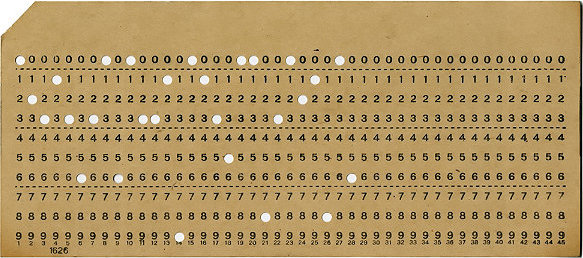
\includegraphics[width=.8\textwidth]{img/punched-card.jpg}

\noindent {\footnotesize (Computer History Museum)}
\end{center}

\begin{itemize}
\item $N$ colunas $\times$ 10 linhas
\item máquina de ordenar cartões: 
\begin{itemize}
  \item configurada com um número de coluna $c$
  \item separa os cartões em 10 caixas em função de qual linha foi perfurada naquela coluna.
  \item o operador junta as pilhas de cartões: furo na 1a posição primeiro, etc.
\end{itemize}
\end{itemize}
\end{frame}

\begin{frame}
  \frametitle{Ordenação \textit{radix sort\/}}
  \framesubtitle{Ideia}
  \begin{itemize}
    \item Como configurar a máquina para ordenar cartões?
      \pause
    \item Solução
      \begin{enumerate}
      \item Separar por dígito menos significativo (unidades)
      \item Juntar
      \item Separar por segundo dígito menos significativo (dezenas)
      \item Juntar
      \item etc. até processar todos os dígitos.
      \end{enumerate}
  \end{itemize}
\end{frame}

\begin{frame}
  \frametitle{Ordenação \textit{radix sort\/}}
  \framesubtitle{Simulação}

  $$
  \begin{array}{c|c|c|c|c}
    \mbox{Inicial} & \mbox{1o dígito} & \mbox{2o dígito} & \mbox{3o dígito} & \mbox{4o dígito} \\
    \hline
    \hline
    \begin{array}{c}
      8091 \\
      0893 \\
      8635 \\
      8805 \\
      8856 \\
      8164 \\
    3868 \\
    9038 \\
    9224
  \end{array}
    &
  \begin{array}{c}
    \only<2->{809\assert{1}} \\
    \only<2->{089\assert{3}} \\
    \only<2->{816\assert{4}} \\
    \only<2->{922\assert{4}} \\
    \only<2->{863\assert{5}} \\
    \only<2->{880\assert{5}} \\
    \only<2->{885\assert{6}} \\
    \only<2->{386\assert{8}} \\
    \only<2->{903\assert{8}}
  \end{array}
  &
  \begin{array}{c}
    \only<3->{88\assert{05}} \\
    \only<3->{92\assert{24}} \\
    \only<3->{86\assert{35}} \\
    \only<3->{90\assert{38}} \\
    \only<3->{88\assert{56}} \\
    \only<3->{81\assert{64}} \\
    \only<3->{38\assert{68}} \\
    \only<3->{80\assert{91}} \\
    \only<3->{08\assert{93}}
  \end{array}
  &
  \begin{array}{c}
    \only<4->{9\assert{038}} \\
    \only<4->{8\assert{091}} \\
    \only<4->{8\assert{164}} \\
    \only<4->{9\assert{224}} \\
    \only<4->{8\assert{635}} \\
    \only<4->{8\assert{805}} \\
    \only<4->{8\assert{856}} \\
    \only<4->{3\assert{868}} \\
    \only<4->{0\assert{893}}
  \end{array}
  &
  \begin{array}{c}
    \only<5>{\assert{0893}} \\
    \only<5>{\assert{3868}} \\
    \only<5>{\assert{8091}} \\
    \only<5>{\assert{8164}} \\
    \only<5>{\assert{8635}} \\
    \only<5>{\assert{8805}} \\
    \only<5>{\assert{8856}} \\
    \only<5>{\assert{9038}} \\
    \only<5>{\assert{9224}}
  \end{array}
  \end{array}
$$

\end{frame}

\begin{frame}
  \frametitle{Ordenação \textit{radix sort\/}}
  \framesubtitle{Algoritmo}

  \begin{codebox}
    \Procname{$\proc{Radix-Sort}(A, d)$}
    \li \For $i \gets 1$ \To $d$
    \li \Do Aplique uma ordenação estável utilizando o dígito $i$
    \zi \End
  \end{codebox}
  \pause
  Observações
  \begin{itemize}
    \item Algoritmo candidato: ordenação por contador
    \item Este algoritmo funciona para qualquer tipo de dados que pode ser visto
      como uma sequência de tamanho fixo ($d$), ordenável
      \alert{lexicograficamente}.
  \end{itemize}
\end{frame}

\begin{frame}
  \frametitle{Ordenação \textit{radix sort\/}}
  \framesubtitle{Análise}

  \begin{description}
  \item[Correção] Verificado por indução utilizando a coluna sendo ordenada, 
    e o fato da ordenação sobre cada coluna ser estável.
  \item[Complexidade] Utilizando a ordenação por contadores, assumindo $k$ dígitos diferentes,
    \begin{itemize}
      \item o custo de cada iteração é $\Theta(n+k)$;
      \item se há $d$ colunas, o custo é $\Theta(d(n+k))$;
      \item quando $d$ é constante, e $k \in O(n)$, então o algoritmo é $\Theta(n)$.
    \end{itemize}
  \end{description}

\end{frame}

\section{Ordenação por lotes}

\begin{frame}
\frametitle{Ordenação por lotes (\textit{bucket sort\/})}
\framesubtitle{Introdução}

\begin{itemize}
  \item Este algoritmo é aplicável quando os dados a serem ordenados
    estão distribuídos \alert{uniformemente} sobre um intervalo.
  \item Intervalo: $\{x \, \mid \, 0 \le x < 1\}$
\end{itemize}

\end{frame}

\begin{frame}
\frametitle{Ordenação por lotes (\textit{bucket sort\/})}
\framesubtitle{Ideia}

\begin{itemize}
  \item Assumindo que há $n$ valores a ordenar;
  \item Criar um arranjo de $n$ listas;
  \item Cada lista armazena os valores em uma parte do intervalo: $0 \le x < 1/n$, $1/n \le x < 2/n$,
    \ldots $n-1/n \le x < 1$.
  \item Os valores a ordenar são inseridos na lista correspondente.
  \item Com alta probabilidade, cada lista é pequena e pode ser processada eficientemente pelo algoritmo de ordenação por inserção
  \item As listas são copiadas para o arranjo final em ordem.
\end{itemize}

\end{frame}

\begin{frame}
\frametitle{Ordenação por lotes (\textit{bucket sort\/})}
\framesubtitle{Ilustração}

\begin{center}
  \includegraphics[width=\textwidth]{fig/bucket-sort.pdf}
\end{center}

\end{frame}

\begin{frame}
\frametitle{Ordenação por lotes (\textit{bucket sort\/})}
\framesubtitle{Algoritmo}

  \begin{codebox}
    \Procname{$\proc{Bucket-Sort}(A)$}
    \li $n \gets \id{length}(A)$
    \li \For $i \gets 1$ \To $n$
    \li \Do Inserir $A[i]$ na lista $B[ \lfloor n \times A[i] \rfloor ]$
    \End
    \li \For $i \gets 0$ \To $n-1$
    \li \Do Ordenar $B[i]$ por inserção
    \End
    \li Concatenar $B[0]$, $B[1]$, \ldots $B[n-1]$, nesta ordem
  \end{codebox}

\end{frame}

\begin{frame}
\frametitle{Ordenação por lotes (\textit{bucket sort\/})}
\framesubtitle{Análise}

\begin{description}
  \item[Correção] \only<2>{
    Considere dois valores $A[i]$ e $A[j]$, tais que $A[i] < A[j]$
    \begin{itemize}
      \item os valores são copiados para os lotes $B[i']$ e $B[j']$, onde:
        \begin{itemize}
          \item $i' = \lfloor n A[i] \rfloor$
          \item $j' = \lfloor n A[j] \rfloor$
          \item Logo $i' \le j'$
        \end{itemize}
      \item se $i' = j'$, então $A[i]$ e $A[j]$ serão ordenados (pois cada lote é ordenado)
      \item se $i' < j'$, então $A[i]$ e $A[j]$ serão ordenados, pois cada valor de $i'$ vem antes de cada valor de $j'$
    \end{itemize}
  }
  \item[Complexidade]
    \only<3>{
    \begin{itemize}
    \item A única parte do algoritmo que tem complexidade linear é a
      ordenação dos lotes (linha 5).
    \item Utilizando resultados da teoria da probabilidade:
      \begin{itemize}
      \item havendo $n$ lotes e $n$ valores, 
      \item assumindo uma distribuição uniforme dos valores no intervalo $[0,1[$
      \item o número esperado de valor por lote é $\Theta(1)$.
    \end{itemize}
    \item O custo esperado de ordenar cada lote é $\Theta(1)$
    \item O custo do algoritmo é linear.
    \end{itemize}
        }
\end{description}

\end{frame}

\section{Síntese}

\begin{frame}
  \frametitle{Síntese}
  \framesubtitle{Algoritmos de ordenação}

  \begin{itemize}
    \item Complexidade teórica: $O(n^2)$ ou $O(n \lg n)$.
    \item Importância da randomização para algoritmos ``quase sempre ótimos''.
    \item Memória auxiliar: constante ou não?
    \item Estabilidade da ordenação.
    \item Características dos dados a serem ordenados
      \begin{itemize}
        \item Completamente aleatórios ou ``quase-ordenados''?
        \item Passíveis de serem tratados por um algoritmo de complexidade linear?
      \end{itemize}
  \end{itemize}
\end{frame}
\end{document}

